% !TEX root = ../arbeit.tex

\chapter{Systems Architecture}
An intuitive to use \ac{PROCAMS} features a tight integration of software and hardware components.
Furthermore, a  fine calibration and well assembled hardware are essential for proficient operation. In the following the architecture design of both, hardware and software, are described in detail.

\section{Hardware Architecture}
The proposed hardware architecture is designed for a compact stand-alone \ac{PROCAMS}. The basis of the systems consists of a camera and a projector. To enable accurate touch detection a depth sensing camera will be used. A motion capture system is no alternative hence it requires an instrumentation of the environment. Such instrumentation would not meet the acquired requirements.
For an easy transformation between the camera and projector coordinate systems, the camera is fixed to the projector. It is important, that the \ac{FOV} of the camera matches the \ac{FOV} of the projector as closely as possible. The projector itself needs to be focus free, as known from laser projectors, or requires the possibility to set the focus electronically via control commands.

Two \ac{DOF} are required to have enough variance to project to any spot visible from the mounting point of the PROCAMS. Thus two rotary actuators are utilised for panning (yaw) and tilting (pitch) of the projector camera unit. The actuator which tilts the unit is bolted directly to the projector. The other is shifted by \SI{90}{\degree} in a vertical plane and bolted to the first actuator. Hereby the projector camera unit is always level. A third actuator which would pivots the unit side to side (roll) is not necessary since it would not change the \emph{interaction space} in a meaningful way.

For a stand-alone solution, the \ac{PROCAMS} includes a powerful processing unit performing all calculations without any remote dependencies. To minimise cable tangle, the processing unit is placed close to the projector and camera. Hence the processing unit is also moving along with the camera and projector. The proposed hardware architecture with a single processing unit for each PROCAMS maximises scalability since no remote connections or calculations are necessary.

An alternative approach using only one powerful dedicated workstation for several PROCAMS is not considered any further. Indeed, the systems could be smaller and lighter since they do not require a processing unit, but this approach will not scale well.
Broadcasting a depth sensing camera video feed for touch detection or elements of the graphical user interface would quickly overstrain the wireless link to the remote unit.

\section{Software Architecture}
Developing a \ac{PROCAMS} fitting the requirements of an average end user is challenging. Technically complex tasks have to be hidden from the user. The initialisation effort has to be minimal while maintaining flexibility. A generic software architecture design for a rotatable \ac{PROCAMS} providing touch input is illustrated in~\autoref{fig:architecture} and described in the following. 

\begin{figure}[htbp] 
   \centering
   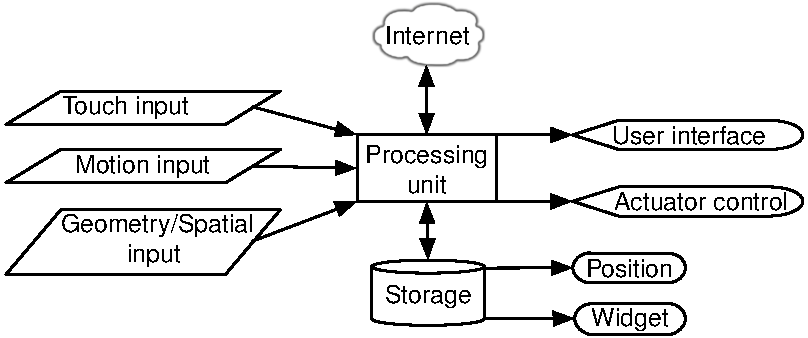
\includegraphics[width=\textwidth]{images/architecture/architecture_noshaddow.pdf} 
   \caption{Generic \acl{PROCAMS} software architecture}
   \label{fig:architecture}
\end{figure}

\paragraph{Processing Unit}
The processing unit is the core piece which includes all logic of the \ac{PROCAMS}.
To provide the desired functionality, it requires three input sources. Touch input to control the \ac{GUI}, motion input to control the pan-tilt unit and finally geometry and spatial input for rectified projection to a defined positions in space.

The main task of the processing unit is to collect all these data and performs the necessary calculations to react like the user intends. For example, touch data are reported to the processing unit in a physical world coordinate system. To trigger events on the corresponding widget, touch events have to be transformed to the \ac{GUI} coordinate system regarding the geometry and spatial input. Moreover, the processing unit takes account of all \emph{displays} and rendered widgets. 
To provide dynamic loading of new content or widgets the  processing unit is wirelessly connected to the Internet.
Furthermore, the wireless link is used for receiving remote motion input which is translated by the processing unit and then forwarded to the actuators to control the pan-tilt unit.

\paragraph{User Interface}
For the end user, the \acl{GUI} is the most important part of the \ac{PROCAMS}. In this architecture design, the \ac{GUI} consists of the actual \emph{surfaces} within the \emph{interaction space} the projector is projecting to. Therefore, it is dynamic in terms of spatial alignment. Within a defined \emph{interaction space} widgets can be placed, moved or removed freely on any \emph{surface}. Since the projector is rotatable, \emph{surfaces} are not always planar to the projector. Hence, widgets are encapsulated in \emph{displays} which pre-warps the content to get a rectified reproduction of the widget rendered onto the surface. Geometrically input is used by the processing unit, to calculate the needed transformation to obtain a rectified projection.

\subparagraph{Touch Input} 
Touch input is provided by new smart phones to interact directly by touching the screen with one or more fingers. 
Nowadays, it is a common and well understood input method for users. To enable touch input on ordinary non instrumented surfaces many \ac{PROCAMS}~\cite{Hardy:2012jo,Wilson:2012fb,Xiao:2013dp} use a depth sensing camera to detect touch. Regardless of how the touch is detected, the world coordinates of the detected touch event are passed to the main processing unit. There they are further processed to trigger the desired interaction.  

\paragraph{Motion Input}
Motion input is used to control the alignment of the \ac{PROCAMS}. In order to define a new \emph{interaction space} motion input needs to be provided externally via remote or touch input. Motion input data is passed to the processing unit which triggers the desired events into control commands. Alternatively, stored configuration can be loaded from the database. Control commands are then directly forward the to the actuators. 

\paragraph{Geometry and Spatial Input}
Geometric and spatial input is necessary to gain geometrically and spatially awareness. Geometrically awareness enables the \ac{PROCAMS} to project rectified \ac{GUI} elements to planar or even nonplanar surfaces. Spatial awareness ensures that stored \ac{GUI} elements are always projected to the same position in space. Geometrical and spatial input can be accomplished via tracking or sensing of the environment, or even a combination of both. 

\paragraph{Actuator Control}
Actuator control commands directly power the actuator which rotates the \ac{PROCAMS} or control the focus of the projector when not focus free. Commands are divided into three individual command segments, which are calculated independently by the processing unit. The tilt command segment controls the rotation of the system in the vertical plane. The range needs to be between \SI{0}{\degree} for horizontal alignment to \SI{90}{\degree} for projection onto the floor. As long as the \ac{PROCAMS} is mounted at the ceiling this range is enough to project to the lower hemisphere. The pan command segment is for rotation in the horizontal plane of the \ac{PROCAMS}. A range of at least \SI{360}{\degree} is necessary to cover the complete hemisphere. 
The processing unit translates the motion input or stored \emph{interaction spaces} alignments into actuator control commands to enable projections to all parts of the space.
If a projector is used which requires manual focusing there is an additional control command segment to keep the projection in focus. The processing unit is required to analyse the spatial and geometrical data input and calculate the correspondent focus actuator command.

\paragraph{Storage}
The storage is directly accessed by the processing unit to store and load content, settings and other properties. In particular widgets and  positions. As already described, widgets are relatively simple and easy to use software components which are loaded into the \ac{GUI}. They can vary from simple clock representation, to interactive information presentation or mini games. The other important information which is stored permanently are \emph{positions}. Positions represent the alignment of the \ac{PROCAMS} for a special use case and are separated in a pan and a tilt component. A position property additionally contains the prior projected widgets and their position within the corresponding \emph{display}.